\documentclass{beamer}
%Information to be included in the title page:
\usetheme{metropolis}

\title{Formula 1 Elo Calculator}
\author{Thomas Hosie}
\date{February 2024}

\begin{document}
\begin{frame}
    \titlepage
\end{frame}

\begin{frame}
    \frametitle{Formula 1}
    Running since 1950, the Formula One World Championship (F1) is the 
\end{frame}

\begin{frame}
    \frametitle{Elo Rating System}
    \begin{itemize}
        \item Developed by Arpad Elo for use in rating chess players.
        \item Each player has a rating assigned to them.
        \item A player with a score 400 points higher is 10 times as likely to win a given match. 
        \item Calculates the expected score between two players.
        \item Then given the actual result, provides an updated rating.
    \end{itemize}
\end{frame}

\begin{frame}
    \frametitle{Elo Rating System Calculation}
    The expected result of a player is given by:
    \begin{center}
        $E_p = \dfrac{1}{1+10^ \dfrac{R_o-R_p}{400}}$
    \end{center}
    The updated Elo of a player is given by:
    \begin{center}
        $R'_p = R_p + K(S_p-E_p)$
    \end{center}
\end{frame}

\begin{frame}
    \frametitle{Elo Rating System Example}
    For a player with Elo of 1400 and opponent with Elo 1800:
    \begin{center}
        $E_p = \dfrac{1}{1+10^ \dfrac{1800-1400}{400}} = \dfrac{1}{1+10^ \dfrac{400}{400}}= \dfrac{1}{1+10^1}= \dfrac{1}{11}= 0.\overline{09}$
    \end{center}
    If the player wins (given a $K$ of 9):
    \begin{center}
        $R'_p = 1400 + 9(1-0.\overline{09})= 1400 + 9(0.\overline{90})= 1400 + 8.\overline{18} \approx 1408$
    \end{center}
\end{frame}

\begin{frame}
    \frametitle{How I Calculated Elo}
    \begin{itemize}
        \item Each race was considered a a series of 1 on 1 races between all drivers competing.
        \item The Elo changes from each 1 on 1 was summed to give a new Elo for each driver.
        \item This was repeated for each race in a given time period.
    \end{itemize}
\end{frame}

\begin{frame}
    \frametitle{Top 10 Maximum Elo All Entries}
    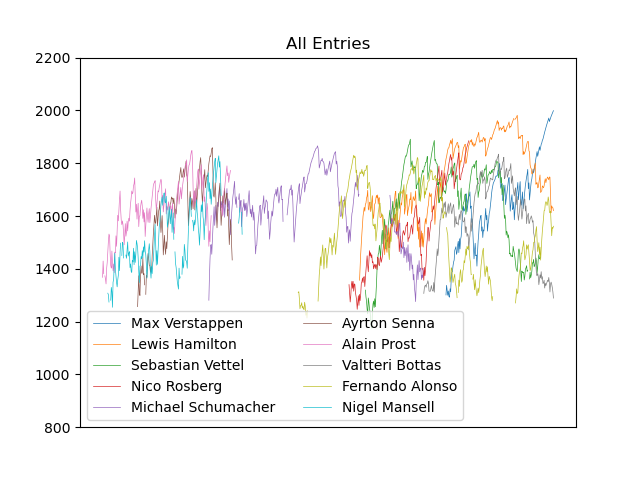
\includegraphics[width=\textwidth]{AllTimeTop10EloAll.png}
\end{frame}

\begin{frame}
    \frametitle{Top 10 Maximum Elo All Finishers}
    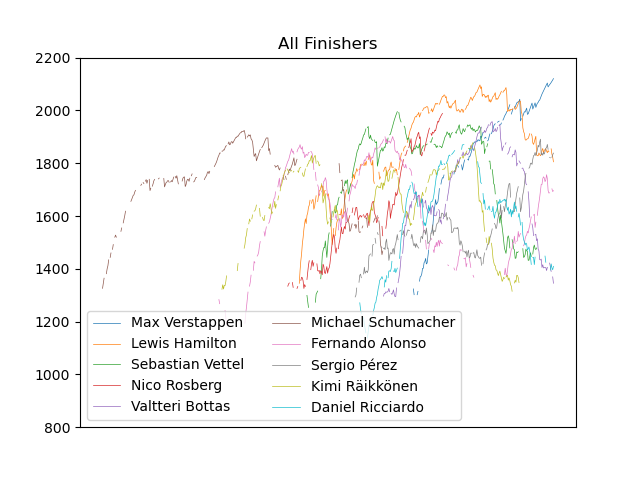
\includegraphics[width=\textwidth]{AllTimeTop10EloFinished.png}
\end{frame}


\begin{frame}
    \frametitle{Issues With The Data}
    \begin{itemize}
        \item For some reason "$\backslash$N" was used as a placeholder.
        \begin{itemize}
            \item Handled by replacing "$\backslash$N" with np.NaN
        \end{itemize}
        \item Before 1961, cars were often shared between drivers.
        \begin{itemize}
            \item Handled by dividing the K value in each 1 on 1 by the number of drivers.
            \item Eg. Car1 with 2 drivers and Car2 with 1, the K values of all interactions would be divided by 2.
        \end{itemize}
    \end{itemize}
\end{frame}

\begin{frame}
    \frametitle{Possible Future Development}
    \begin{itemize}
        \item Analyse the effect of more races in a season.
        \begin{itemize}
            \item Perhaps vary the K value of each interaction by the number of races in a season.
        \end{itemize}
        \item Create a way to factor in the relative performance of different cars.
        \item Investigate the case of inflation of the Elo values over time. 
    \end{itemize}
\end{frame}


\begin{frame}
    \frametitle{Thanks}
    \begin{center}
        All data was taken from CSV's found at ergast.com and checked against other sources for accuracy.
    
        \LARGE{Any Questions?}
    \end{center}
\end{frame}

\end{document}